\section{Experimental Methodology}
\label{methodology}
\subsection{System Setup}
In this study, the target machine is a Creality CR-10 V3 3D printer featuring an XZ-head architecture, while the visual sensor for the virtual encoder system is an OV9821 camera module operating at a resolution of $1280 \times 720$ pixels at 120 frames per second. To interface the camera with the machine, a custom PLA camera mount is employed. The camera is mounted directly on the X-carriage width with a fixed height of 260 mm from the print bed. The camera is placed to capture the displacement of a chessboard marker affixed to the Y-axis print bed. The visualization of the system setup is illustrated in \figref{fig:setup}. 

\begin{figure}[ht]
    \centering
    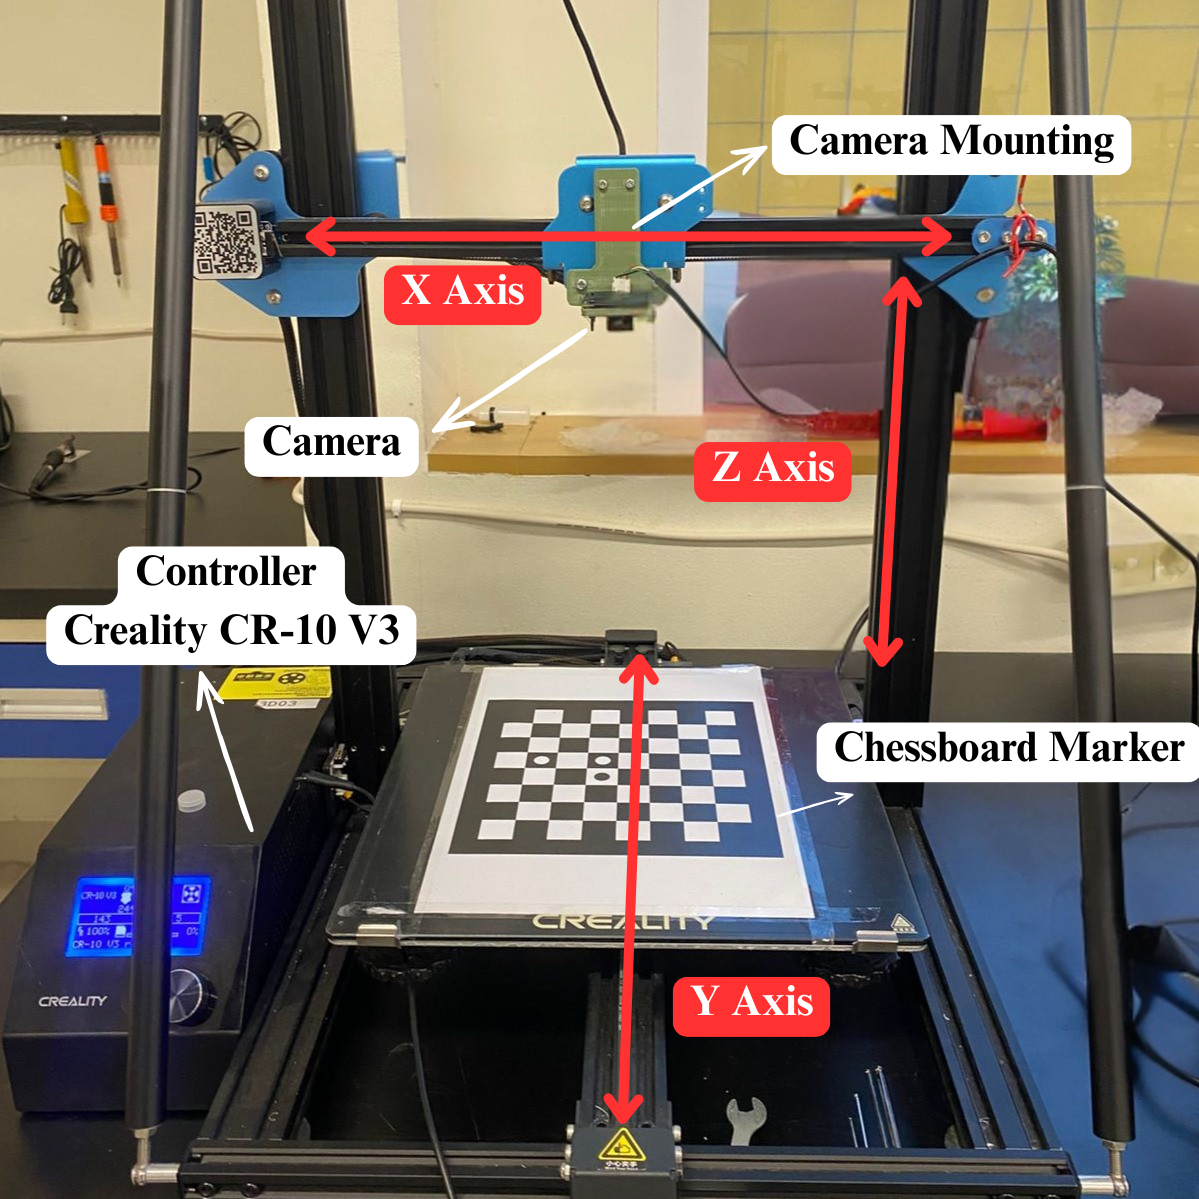
\includegraphics[width=0.75\linewidth]{images/setup.png}
    \caption{System Setup Configuration}
    \label{fig:setup}
\end{figure}

The specifications of the displayed chessboard marker are detailed as follows: 
\begin{enumerate}
    \item Calibration Board: A single calibration target featuring an $8 \times 8$ chessboard grid with a square size of 20 mm.
    \item Sorting Anchors: Three circular marker anchors with a radius of 5 mm positioned at the center of the board.
    \item Reference Specifications: Adopted from the benchmark parameters defined in \cite{Dan2022}.
\end{enumerate}


\subsection{Camera Calibration}


Prior to deploying the camera-based virtual encoder system, camera calibration must be conducted to establish baseline geometric parameters. The calibration workflow is partitioned into three main stages: Feature Extraction utilizing the EDLines algorithm, Homography Alignment to resolve chessboard orientation, and Calibration Evaluation to extract the camera intrinsic matrix, distortion coefficients, and overall reprojection error. The complete camera calibration procedure is summarized in Algorithm \ref{alg:calibration_pipeline}.

%%%%%%%% ini dihapus
\begin{algorithm}[t]
\caption{Camera Calibration Pipeline}
\label{alg:calibration_pipeline}
\begin{algorithmic}[1]
\footnotesize

\Function{FeatureExtraction}{$I_{\text{gray}}$}
    \State $L_{\text{raw}} \gets \text{EDLines}(I_{\text{gray}})$
    \State $C_{\text{init}}, L_{\text{valid}} \gets \text{ScreenLinesAndIntersect}(I_{\text{gray}}, L_{\text{raw}})$
    \State $C_{\text{sub}} \gets \text{SubpixelOptimization}(I_{\text{gray}}, C_{\text{init}})$
    \State \Return $C_{\text{sub}}$
\EndFunction

\Statex

\Function{HomographyAlignment}{$C_{\text{sub}}, I_{\text{gray}}, (M, N)$}
    \State $I_{\text{enh}} \gets \text{GaussianBlur}(\text{CLAHE}(I_{\text{gray}}), (5,5))$
    \State $E \gets \text{DetectEllipsesOrCircles}(I_{\text{enh}})$
    \State $C_{\text{grid}} \gets \text{FilterCentralPoints}(C_{\text{sub}}, E, M \times N)$
    \State $idx_{TL} \gets \arg\min(x+y)$
    \State $idx_{BR} \gets \arg\max(x+y)$
    \State $idx_{TR} \gets \arg\max(x-y)$
    \State $idx_{BL} \gets \arg\min(x-y)$
    \State $P_{\text{src}} \gets [C_{\text{grid}}[idx_{TL}], C_{\text{grid}}[idx_{TR}],$
    \Statex \hspace{3.5em} $C_{\text{grid}}[idx_{BR}], C_{\text{grid}}[idx_{BL}]]$
    \State $P_{\text{dst}} \gets [(0,0), (M-1,0), (M-1,N-1), (0,N-1)]$
    \State $H \gets \text{FindHomography}(P_{\text{dst}}, P_{\text{src}})$
    \State $C_{\text{sorted}} \gets \text{SnapGridToPoints}(C_{\text{grid}}, H, M, N)$
    \State \Return $C_{\text{sorted}}$
\EndFunction

\Statex

\Function{CalibrationEvaluation}{$\{\mathcal{P}_{3D}\}, \{\mathcal{C}_{2D}\}, \text{shape}$}
    \State $K, D, \{R_i\}, \{t_i\} \gets \text{CalibrateCamera}($
    \Statex \hspace{4em} $\{\mathcal{P}_{3D}\}, \{\mathcal{C}_{2D}\}, \text{shape})$
    \State $\text{SSE}_{\text{total}} \gets 0, \quad N_{\text{total}} \gets 0$
    \For{$i = 1 \dots |\mathcal{C}_{2D}|$}
        \State $\hat{p}_i \gets \text{ProjectPoints}(\mathcal{P}_{3D}[i], R_i, t_i, K, D)$
        \State $\text{SSE}_i \gets \|\mathcal{C}_{2D}[i] - \hat{p}_i\|_2^2$
        \State $\text{SSE}_{\text{total}} \gets \text{SSE}_{\text{total}} + \text{SSE}_i$
        \State $N_{\text{total}} \gets N_{\text{total}} + N_{\text{pts}}$
    \EndFor
    \State $\text{RMSE}_{\text{overall}} \gets \sqrt{\text{SSE}_{\text{total}} / N_{\text{total}}}$
    \State \Return $K, D, \text{RMSE}_{\text{overall}}$
\EndFunction

\Statex
\textbf{Main Execution Routine:}
\State Initialize $\mathcal{C}_{2D} \gets \emptyset$, $\mathcal{P}_{3D} \gets \emptyset$
\For{each image $I \in \text{Dataset}$}
    \State $I_{\text{gray}} \gets \text{ConvertToGray}(I)$
    \State $C_{\text{sub}} \gets \text{FeatureExtraction}(I_{\text{gray}})$
    \State $C_{\text{sorted}} \gets \text{HomographyAlignment}($
    \Statex \hspace{5.5em} $C_{\text{sub}}, I_{\text{gray}}, (M, N))$
    \If{$C_{\text{sorted}} \neq \text{None}$}
        \State Append $\mathcal{P}_{3D}$ and $C_{\text{sorted}}$ to $\{\mathcal{P}_{3D}\}$ and $\{\mathcal{C}_{2D}\}$
    \EndIf
\EndFor
\State $K, D, \text{RMSE}_{\text{overall}} \gets \text{CalibrationEvaluation}($
\Statex \hspace{4em} $\{\mathcal{P}_{3D}\}, \{\mathcal{C}_{2D}\}, \text{shape})$

\end{algorithmic}
\end{algorithm}

%%%%%%% dijadikan paragraf


\subsection{Virtual Encoder Workflow}
As outlined in Section \ref{proposed_encoder}, the virtual encoder leverages EDLines-based feature extraction—identical to the camera calibration pipeline—to extract precise chessboard corner coordinates. These refined corner points are subsequently utilized for 6-DOF pose estimation to track the relative spatial displacement of the chessboard marker across sequential image frames with respect to the camera frame. Pose estimation is resolved using an iterative Perspective-n-Point (SolvePnP) solver. The complete virtual encoder procedure is detailed in Algorithm \ref{alg:pose_extraction}.

\begin{algorithm}[t]
\caption{Virtual Encoder Workflow}
\label{alg:pose_extraction}
\begin{algorithmic}[1]
\footnotesize

\Require Image $I$, Intrinsic $\mathbf{K}$, Distortion $\mathbf{D}$, 3D points $\mathbf{P}_{3\text{D}}$,
\Statex \hspace{2.5em} Grid $(W, H) = (7, 7)$, Threshold $\epsilon_{\text{rmse}}$
\Ensure Position $p = (p_{\text{active}}, p_{\text{passive}})$, Error $\epsilon$

\Function{ExtractPosition}{$I, \mathbf{K}, \mathbf{D}, \mathbf{P}_{3\text{D}}$}
    \If{$I$ is invalid or empty} 
        \State \Return $\text{Null}, \infty$ 
    \EndIf

    \State $I_{\text{gray}} \gets \text{ConvertToGrayscale}(I)$
    \State $C_{\text{sub}} \gets \text{FeatureExtraction}(I_{\text{gray}})$
    \State $C_{\text{sorted}} \gets \text{HomographyAlignment}($
    \Statex \hspace{5.5em} $C_{\text{sub}}, I_{\text{gray}}, (W, H))$

    \If{$C_{\text{sorted}} = \text{Null}$}
        \State \Return $\text{Null}, \infty$
    \EndIf

    \State $\text{success}, \mathbf{rvec}, \mathbf{tvec} \gets \text{SolvePnP}(\mathbf{P}_{3\text{D}}, C_{\text{sorted}}, \mathbf{K}, \mathbf{D})$

    \If{$\text{success}$}
        \State $\mathbf{P}_{\text{proj}} \gets \text{ProjectPoints}(\mathbf{P}_{3\text{D}}, \mathbf{rvec}, \mathbf{tvec}, \mathbf{K}, \mathbf{D})$
        \State $\epsilon \gets \sqrt{\frac{1}{M} \|C_{\text{sorted}} - \mathbf{P}_{\text{proj}}\|_2^2}$

        \If{$\epsilon \le \epsilon_{\text{rmse}}$}
            \State Extract 2D translation $p \gets (\mathbf{tvec}[0], \mathbf{tvec}[1])$
            \State \Return $p, \epsilon$
        \EndIf
    \EndIf

    \State \Return $\text{Null}, \infty$
\EndFunction

\end{algorithmic}
\end{algorithm}

\subsection{Virtual Encoder Measurement Error Testing and Metrological Framework}
In this stage, the measurement accuracy of the virtual encoder system is evaluated by comparing its displacement readouts against reference measurements obtained using a high-precision mechanical dial gauge. The physical machine movement sequence employed for this evaluation is described in Algorithm \ref{alg:sequence}.

\begin{algorithm}[t]
	\caption{Data Capturing Sequence for Kinematic Error Extraction}
	\label{alg:sequence}
	\begin{algorithmic}[1]
		\footnotesize
		
		\Require Commanded displacement $D_{\text{cmd}}$, total iterations $N$
		\Ensure Captured frames $\mathcal{F} = \{F_{\text{init}, i}, F_{\text{fwd}, i}, F_{\text{rev}, i}\}$ and
		\Statex \hspace{2.5em} positions $\{p_{\text{init}, i}, p_{\text{fwd}, i}, p_{\text{rev}, i}\}$
		
		\State Move machine active axis to reference anchor position $p_0$
		\State Capture Initial Frame $F_{\text{init}, 1} \implies p_{\text{init}, 1}$
		
		\For{$i = 1$ \textbf{to} $N$}
		\State Move Forward by $+D_{\text{cmd}}$
		\State Capture Forward Frame $F_{\text{fwd}, i} \implies p_{\text{fwd}, i}$
		\State Move Backward by $-D_{\text{cmd}}$
		\State Capture Reversal Frame $F_{\text{rev}, i} \implies p_{\text{rev}, i}$
		\If{$i < N$}
		\State Perform Preload Out (Move $-D_{\text{cmd}}$)
		\State Perform Preload In (Move $+D_{\text{cmd}}$)
		\State Capture Initial Frame $F_{\text{init}, i+1} \implies p_{\text{init}, i+1}$
		\EndIf
		\EndFor
		
	\end{algorithmic}
\end{algorithm}

For this evaluation sequence, a commanded displacement ($D_{\text{cmd}}$) of 0.5~mm is selected, conforming to the physical travel limits of the dial gauge, which features a maximum single-revolution range of 0.8~mm. Positional readouts extracted from the forward and reversal frames are subsequently compared, and their mean deviation is calculated to determine the absolute measurement error of the virtual encoder.

To establish a rigorous metrological foundation, a measurement uncertainty framework is formulated in accordance with the ISO/IEC Guide 98-3 (GUM) standard. The combined standard uncertainty ($u_c$) incorporates both Type A evaluations (derived from statistical experimental repeatability) and Type B evaluations (derived from systemic physical, optical, and hardware boundaries). The combined uncertainty model is expressed analytically as:
\begin{equation}
	u_c = \sqrt{u_A^2 + u_{\text{noise}}^2 + u_{\text{reproj}}^2 + u_{\text{dial}}^2}
	\label{eq:gum_uc}
\end{equation}
where:
\begin{itemize}
	\item $u_A = \frac{\sigma}{\sqrt{N}}$ defines the Type A standard uncertainty from $N$ repeated displacement measurements.
	\item $u_{\text{noise}}$ denotes the Type B standard uncertainty induced by static optical fluctuations and mechanical micro-vibrations.
	\item $u_{\text{reproj}}$ quantifies the sub-pixel reprojection residual uncertainty, modeled across the spatial averaging of the $7 \times 7$ chessboard corner grid.
	\item $u_{\text{dial}} = \frac{a}{\sqrt{3}}$ represents the Type B uncertainty from the reference dial gauge tolerance ($a = 10~\mu\text{m}$), assuming a uniform rectangular distribution.
\end{itemize}

The expanded uncertainty ($U$) at a 95\% confidence level is subsequently evaluated using a coverage factor of $k = 2$:
\begin{equation}
	U = k \cdot u_c = 2 \cdot u_c
	\label{eq:gum_expanded}
\end{equation}

\subsection{Machine Calibration Protocol}
The proposed calibration framework comprises three distinct evaluation phases: Measurement Error, Linear Axis Error, and Circular Trajectory Error profiling. Both linear axis and circular trajectory performance are evaluated under baseline (uncalibrated) conditions and post-calibration states to verify compensation effectiveness. The overall calibration protocol workflow is illustrated in \figref{fig:protocol}.

\begin{figure}[ht]
    \centering
    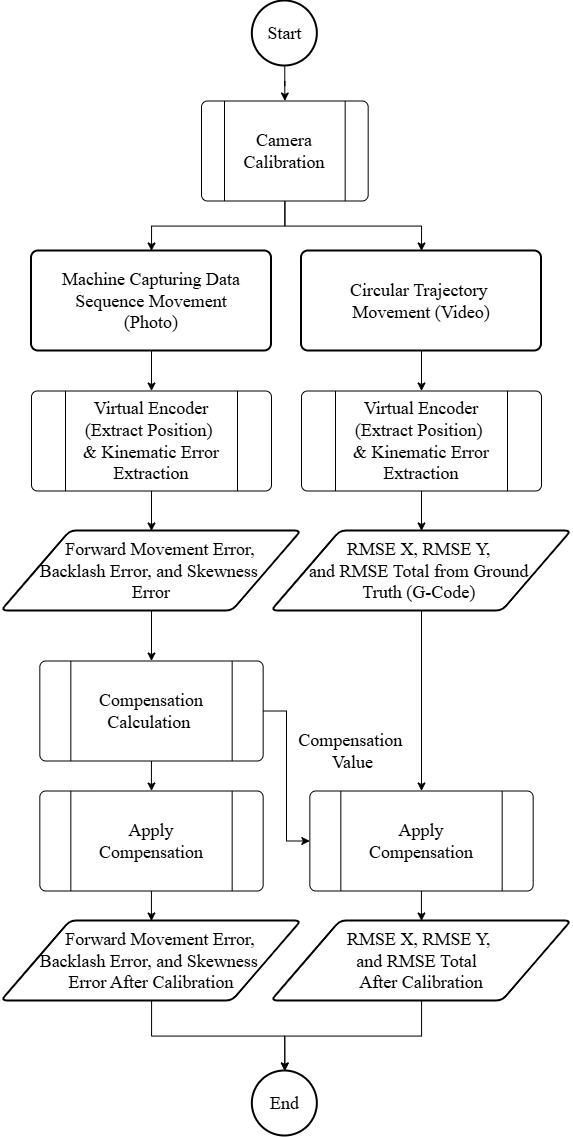
\includegraphics[width=0.75\linewidth]{images/Calibration Protocol Fix.drawio.png}
    \caption{Calibration Protocol Diagram}
    \label{fig:protocol}
\end{figure}

\begin{algorithm}[t]
	\caption{Kinematic Parameter Extraction and Compensation}
	\label{alg:kompensasi}
	\begin{algorithmic}[1]
		\footnotesize
		
		\Function{KinematicErrorExtraction}{$\mathcal{S}, \mathbf{K}, \mathbf{D}, \mathbf{P}_{3\text{D}}, \epsilon_{\text{thresh}}, N_{\text{max}}$}
		\State Initialize $\mathcal{D}_{\text{act}} \gets \emptyset$, $\mathcal{B} \gets \emptyset$, $\mathcal{S}_{\text{skew}} \gets \emptyset$, $N_{\text{valid}} \gets 0$
		
		\For{each triplet $(F_{\text{init}}, F_{\text{fwd}}, F_{\text{rev}}) \in \mathcal{S}$}
		\State $p_{\text{init}}, \epsilon_{\text{init}} \gets \text{ExtractPosition}(F_{\text{init}}, \mathbf{K}, \mathbf{D}, \mathbf{P}_{3\text{D}})$
		\State $p_{\text{fwd}}, \epsilon_{\text{fwd}} \gets \text{ExtractPosition}(F_{\text{fwd}}, \mathbf{K}, \mathbf{D}, \mathbf{P}_{3\text{D}})$
		\State $p_{\text{rev}}, \epsilon_{\text{rev}} \gets \text{ExtractPosition}(F_{\text{rev}}, \mathbf{K}, \mathbf{D}, \mathbf{P}_{3\text{D}})$
		
		\State $\epsilon_{\text{max}} \gets \max(\epsilon_{\text{init}}, \epsilon_{\text{fwd}}, \epsilon_{\text{rev}})$
		\If{$p_{\text{init}} \neq \text{Null} \land p_{\text{fwd}} \neq \text{Null} \land p_{\text{rev}} \neq \text{Null} \land \epsilon_{\text{max}} \le \epsilon_{\text{thresh}}$}
		\State $\Delta p_{\text{act}} \gets p_{\text{fwd,act}} - p_{\text{init,act}}$
		\State $\Delta p_{\text{pas}} \gets p_{\text{fwd,pas}} - p_{\text{init,pas}}$
		\State $B_i \gets |p_{\text{rev,act}} - p_{\text{init,act}}|$
		\State $S_i \gets \Delta p_{\text{pas}} / \Delta p_{\text{act}}$
		
		\State Append $\Delta p_{\text{act}}$ to $\mathcal{D}_{\text{act}}$, $B_i$ to $\mathcal{B}$, $S_i$ to $\mathcal{S}_{\text{skew}}$
		\State $N_{\text{valid}} \gets N_{\text{valid}} + 1$
		
		\If{$N_{\text{valid}} \ge N_{\text{max}}$}
		\State \textbf{break}
		\EndIf
		\EndIf
		\EndFor
		\State \Return $\mathcal{D}_{\text{act}}, \mathcal{B}, \mathcal{S}_{\text{skew}}$
		\EndFunction
		
		\Statex
		
		\Function{CompensationCalculation}{$\mathcal{D}_{\text{act}}, \mathcal{B}, \mathcal{S}_{\text{skew}}, D_{\text{cmd}}, S_{\text{curr}}$}
		\If{$\mathcal{D}_{\text{act}} = \emptyset$}
		\State \Return $\text{Null}, \text{Null}, \text{Null}$
		\EndIf
		
		\State $\bar{\Delta p}_{\text{act}} \gets \text{Mean}(\mathcal{D}_{\text{act}})$
		\State $\bar{B} \gets \text{Mean}(\mathcal{B})$
		\State $\bar{S} \gets \text{Mean}(\mathcal{S}_{\text{skew}})$
		
		\State $S_{\text{new}} \gets (D_{\text{cmd}} / \bar{\Delta p}_{\text{act}}) \cdot S_{\text{curr}}$
		\State $B_{\text{comp}} \gets \bar{B}$
		\State $I_{\text{skew}} \gets \bar{S}$
		
		\State \Return $S_{\text{new}}, B_{\text{comp}}, I_{\text{skew}}$
		\EndFunction
		
		\Statex
		
		\Function{ApplyCompensation}{$\mathbf{p}, A, \mathbf{\Theta}, b$}
		\State Extract $(\Delta x, \Delta y) \gets \mathbf{p}$ and $(S_{\text{new}}, B_{\text{comp}}, I_{\text{skew}}) \gets \mathbf{\Theta}$
		\If{$S_{\text{new}} \neq \text{Null}$}
		\State Send G-code: \texttt{M92} $A = S_{\text{new}}$
		\EndIf
		
		\State $\Delta x_{\text{comp}} \gets \Delta x, \quad \Delta y_{\text{comp}} \gets \Delta y$
		
		\If{$A = X$}
		\State $\Delta y_{\text{comp}} \gets \Delta y_{\text{comp}} - (\Delta x \cdot I_{\text{skew}})$
		\ElsIf{$A = Y$}
		\State $\Delta x_{\text{comp}} \gets \Delta x_{\text{comp}} - (\Delta y \cdot I_{\text{skew}})$
		\EndIf
		
		\If{$b = \text{True}$}
		\If{$A = X$}
		\If{$\Delta x_{\text{comp}} < 0$}
		\State $\Delta x_{\text{comp}} \gets \Delta x_{\text{comp}} - B_{\text{comp}}$
		\Else
		\State $\Delta x_{\text{comp}} \gets \Delta x_{\text{comp}} + B_{\text{comp}}$
		\EndIf
		\ElsIf{$A = Y$}
		\If{$\Delta y_{\text{comp}} < 0$}
		\State $\Delta y_{\text{comp}} \gets \Delta y_{\text{comp}} - B_{\text{comp}}$
		\Else
		\State $\Delta y_{\text{comp}} \gets \Delta y_{\text{comp}} + B_{\text{comp}}$
		\EndIf
		\EndIf
		\EndIf
		
		\State \Return $\Delta x_{\text{comp}}, \Delta y_{\text{comp}}$
		\EndFunction
		
	\end{algorithmic}
\end{algorithm}

\subsection{Machine Linear Movement Performance Examination}
To extract linear step drift, mechanical backlash, and structural axis skewness error, this research utilizes a structured machine movement sequence to capture three distinct types of optical image frames, as detailed before in Algorithm~\ref{alg:sequence}:
\begin{enumerate}
    \item Initial Frame ($F_{\text{init}}$): Captured at the starting reference anchor coordinate, yielding the baseline spatial position $p_{\text{init}}$.
    \item Forward Frame ($F_{\text{fwd}}$): Captured after executing a forward displacement along the active axis, yielding the forward coordinate $p_{\text{fwd}}$.
    \item Reversal Frame ($F_{\text{rev}}$): Captured after returning to the nominal initial position, yielding the post-reversal coordinate $p_{\text{rev}}$.
\end{enumerate}
The measured spatial positions ($p_{\text{init}}$, $p_{\text{fwd}}$, and $p_{\text{rev}}$) extracted from these captured frames are subsequently used to compute the steps per millimeter correction, mechanical backlash, and axis skew factor. 

Prior to parameter aggregation, each image triplet undergoes strict outlier filtering based on the reprojection error threshold $\epsilon_{\text{rmse}}$. Valid position measurements are subsequently processed to isolate individual error metrics across $N_{\text{valid}}$ valid iterations. The analytical formulation for updating the steps-per-millimeter resolution, mechanical backlash compensation, and axis skew factor is formalized in Algorithm \ref{alg:kompensasi}. To obtain optimal parameters during the calibration process, fine-tuning is performed by repeating the same process until the machine reaches a steady state.

\subsection{Machine Circular Movement Performance Examination}
Because real-world additive manufacturing operations require coordinated multi-axis motion rather than single-axis displacements, evaluating tracking performance along continuous paths is essential for comprehensive machine profiling. To assess dynamic synchronization, a complex elliptical trajectory is executed, as depicted in \figref{fig:circexam}. The machine traces the commanded path via G-code execution while the virtual encoder records positional states at each video frame. The tracked trajectory is subsequently benchmarked against the ground-truth path using Root Mean Square Error (RMSE) analysis. The algorithmic workflow for this tracking evaluation is detailed in Algorithm \ref{alg:circular_eval}.

\begin{figure}[ht]
    \centering
    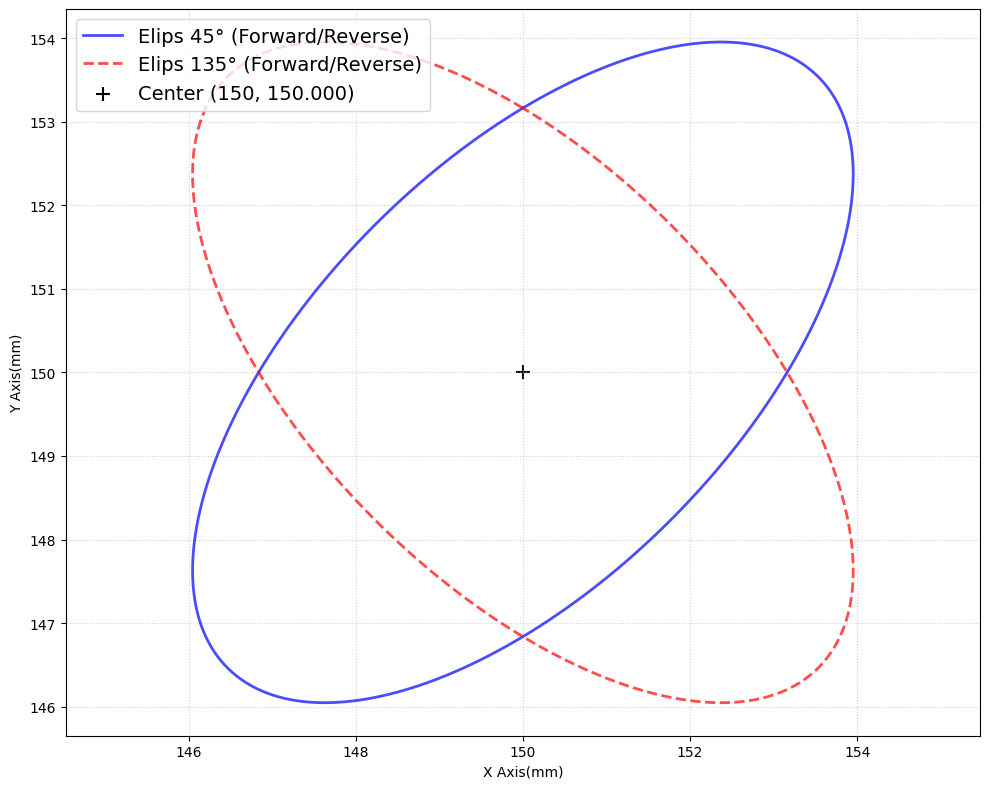
\includegraphics[width=0.8\linewidth]{images/circularmovement.png}
    \caption{Circular Examination Ellipse Model}
    \label{fig:circexam}
\end{figure}

\begin{algorithm}[t]
\caption{Circular Trajectory Extraction and Evaluation}
\label{alg:circular_eval}
\begin{algorithmic}[1]
\footnotesize

\Function{TrajectoryEvaluation}{$\mathcal{V}_{\text{dataset}}, \mathbf{P}_{\text{gt}}, \mathbf{K}, \mathbf{D}, \mathbf{P}_{3\text{D}}, \epsilon_{\text{thresh}}$}
    \State $T_{\text{gt}} \gets \text{BuildKDTree}(\mathbf{P}_{\text{gt}})$ \Comment{Build spatial tree index}
    \State Initialize $\mathcal{E}_x \gets \emptyset, \mathcal{E}_y \gets \emptyset, \mathcal{E}_{\text{tot}} \gets \emptyset$

    \For{each video $V \in \mathcal{V}_{\text{dataset}}$}
        \State Initialize $\mathbf{P}_{\text{enc}} \gets \emptyset$, $p_0 \gets \text{Null}$

        \State \Comment{1. Frame-by-Frame Virtual Encoder Trajectory Extraction}
        \For{each frame $I_k \in V$}
            \State $p_k, \epsilon_k \gets \text{ExtractPosition}(I_k, \mathbf{K}, \mathbf{D}, \mathbf{P}_{3\text{D}})$

            \If{$p_k \neq \text{Null} \land \epsilon_k \le \epsilon_{\text{thresh}}$}
                \If{$p_0 = \text{Null}$}
                    \State $p_0 \gets p_k$ \Comment{Set baseline origin}
                \EndIf
                \State $\mathbf{p}_{\text{rel}} \gets p_k - p_0$ \Comment{Compute relative displacement}
                \State Append $\mathbf{p}_{\text{rel}} \to \mathbf{P}_{\text{enc}}$
            \EndIf
        \EndFor

        \State Export $\mathbf{P}_{\text{enc}}$ to CSV \Comment{Save extracted trajectory}

        \State \Comment{2. Trajectory Tracking Evaluation}
        \State $\mathbf{P}_{\text{enc}} \gets \mathbf{P}_{\text{enc}} - \mathbf{P}_{\text{enc}}[0] + \mathbf{P}_{\text{gt}}[0]$ \Comment{Align initial origin}
        \State $\mathbf{P}_{\text{cls}}, \mathbf{d} \gets \text{QueryNearest}(T_{\text{gt}}, \mathbf{P}_{\text{enc}})$ \Comment{Nearest-neighbor search}

        \State $e_x \gets \sqrt{\text{Mean}((\mathbf{P}_{\text{enc}, x} - \mathbf{P}_{\text{cls}, x})^2)} \times 1000$
        \State $e_y \gets \sqrt{\text{Mean}((\mathbf{P}_{\text{enc}, y} - \mathbf{P}_{\text{cls}, y})^2)} \times 1000$
        \State $e_{\text{tot}} \gets \sqrt{\text{Mean}(\mathbf{d}^2)} \times 1000$

        \State Append $e_x \to \mathcal{E}_x, \quad e_y \to \mathcal{E}_y, \quad e_{\text{tot}} \to \mathcal{E}_{\text{tot}}$
    \EndFor

    \State $\bar{E}_x \gets \text{Mean}(\mathcal{E}_x), \quad \bar{E}_y \gets \text{Mean}(\mathcal{E}_y), \quad \bar{E}_{\text{tot}} \gets \text{Mean}(\mathcal{E}_{\text{tot}})$
    \State \Return $\bar{E}_x, \bar{E}_y, \bar{E}_{\text{tot}}$ \Comment{RMSE in $\mu\text{m}$}
\EndFunction

\end{algorithmic}
\end{algorithm}